-\begin{center}
\textsc{\Large Laboratorio 3}~\\
{\large Vídeo Juegos, Programación}~\\
\emph{Sprites}
\end{center}

\section{Pre-Laboratorio}
\begin{itemize}
\item Investigar los siguientes conceptos:
\begin{enumerate}
  \item Texturas (en cuanto a computación gráfica).
  \item Planos o quads.
  \item Rasterizacion de triangulos.
  \item Matrices de proyección, vista y modelo (projection matrix, view matrix, model matrix)
  \item Espacio de camara, de mundo, de objeto y de pantalla (camera space, world space, object space, screen space)
\end{enumerate}
\end{itemize}
\section{Definición}
\setlength\intextsep{0pt}
\begin{wrapfigure}[12]{l}{0.15\linewidth}

\includegraphics[width=\linewidth]{semana3/sprite_ej1.png} 
\caption{\emph{Sprite} de una unidad en Battle for Wesnoth \cite{wesnothgame}}
\end{wrapfigure}

En computación gráfica un \emph{sprite} es una imagen 2D o animación que es utilizada en una escena.

Los \emph{sprites} fueron originalmente inventados como un método rápido de composición entre varias imágenes en vídeo juegos 2D utilizando hardware especializado. A medida que el performance de los computadores mejoro esta optimización se convirtió innecesario y el termino \emph{sprites} hoy día se refiere específicamente a imágenes 2D que son integradas o utilizadas en una escena \cite{sprites_siggraph}.

Ahora usualmente \emph{sprite} se refiere a imágenes 2D parcialmente transparentes que son proyectadas a un plano en una escena 3D o 2D.~\\[1cm]
\begin{figure}[H]
\centering
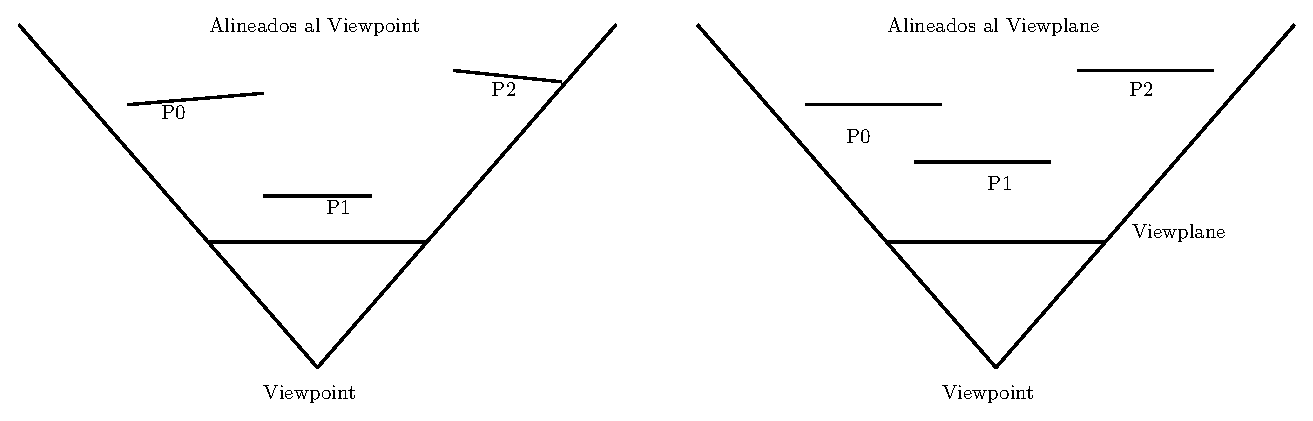
\includegraphics[width=0.95\linewidth]{semana3/bills.eps} 
\caption{Tecnicas para alinear planos sprites}
\end{figure}

\section{Actividad}
\todo[inline]{Por hacer.}
